\documentclass[conference]{IEEEtran}
\usepackage{hyperref}
\usepackage{graphics} % Required for the inclusion of images
\usepackage{graphicx} % Required for the inclusion of images
\usepackage{leftidx}
\usepackage{caption}
\usepackage[flushleft]{threeparttable}
\usepackage{amssymb}
\usepackage{tabularx}
\usepackage{amsmath}
\usepackage{subfigure}
\usepackage{pifont}
\usepackage{tikz}
\usepackage{pgfplots}
\usepackage{textcomp}
\usepackage{standalone}
\usepackage{import}
\usepackage{environ}
\usepackage{lipsum}
\usepackage[ruled,linesnumbered]{algorithm2e}
\usepackage{xcolor}
\usepgfplotslibrary{fillbetween}
\usetikzlibrary{patterns}
\usetikzlibrary{calc}
\newcommand{\blue}[1]{\textcolor{blue}{#1}}
\newcommand{\red}[1]{\textcolor{red}{#1}}

\title{\LaTeX\, Gallery}

\author{
    \IEEEauthorblockN{Junyan Su}
    \IEEEauthorblockA{junyan.su@my.cityu.edu.hk}
}

\begin{document}
\maketitle

\begin{abstract}
    This is a small gallery of latex examples. I found some good figures/tables in the literature and reproduce them with latex. Every example corresponds to a standalone tex file in the folder submodules. A github repository is also available\footnote{\url{https://github.com/sujunyan/tex-gallery}}.
\end{abstract}


\begin{IEEEkeywords}
    \LaTeX , Figure, Table
\end{IEEEkeywords}

\section{Introduction}
% figure 2a/2b ----------------------
\lipsum
\begin{figure}[tb]
      \centering
      %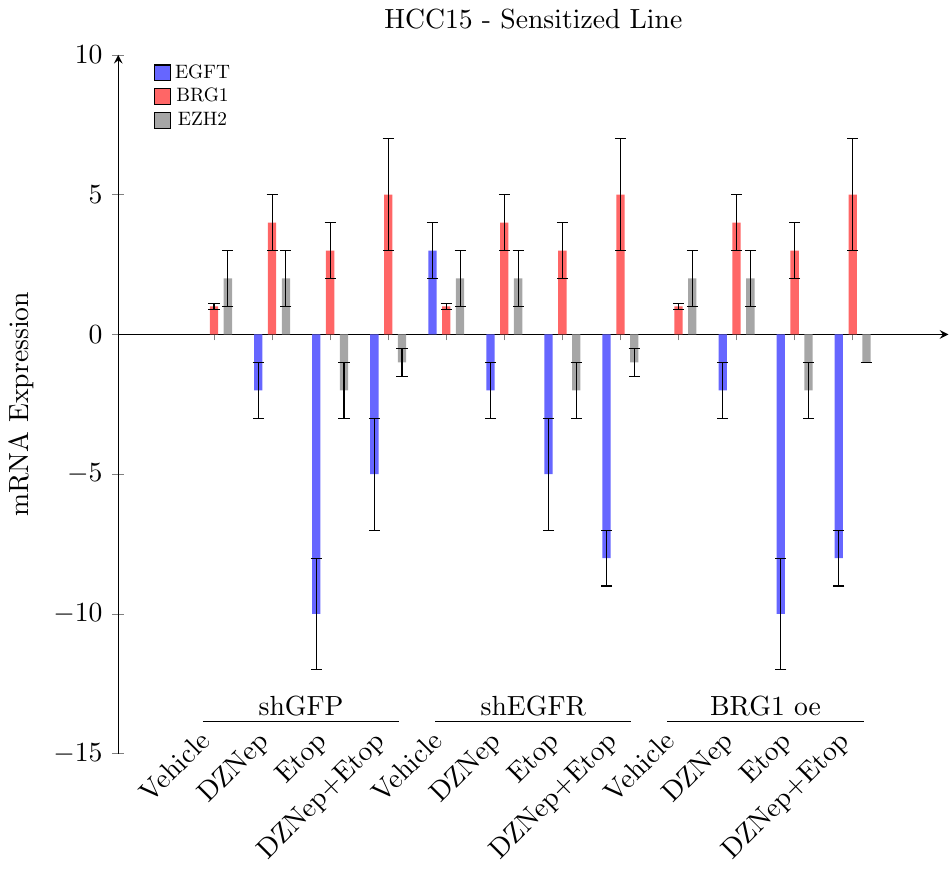
\includegraphics[width=\linewidth]{submodules/2a/2a.pdf}
      %\documentclass[tikz]{standalone}
%\usepackage{pgfplots}
% the figures style are inspired by \url{https://www.nature.com/articles/nature14122/figures/12}.
% For the use of draw group line, refer to https://tex.stackexchange.com/questions/55554/how-can-i-mix-an-ybar-and-an-ybar-stacked-with-pgfplots
%\begin{document}



% figure a -------------------------------------------------------


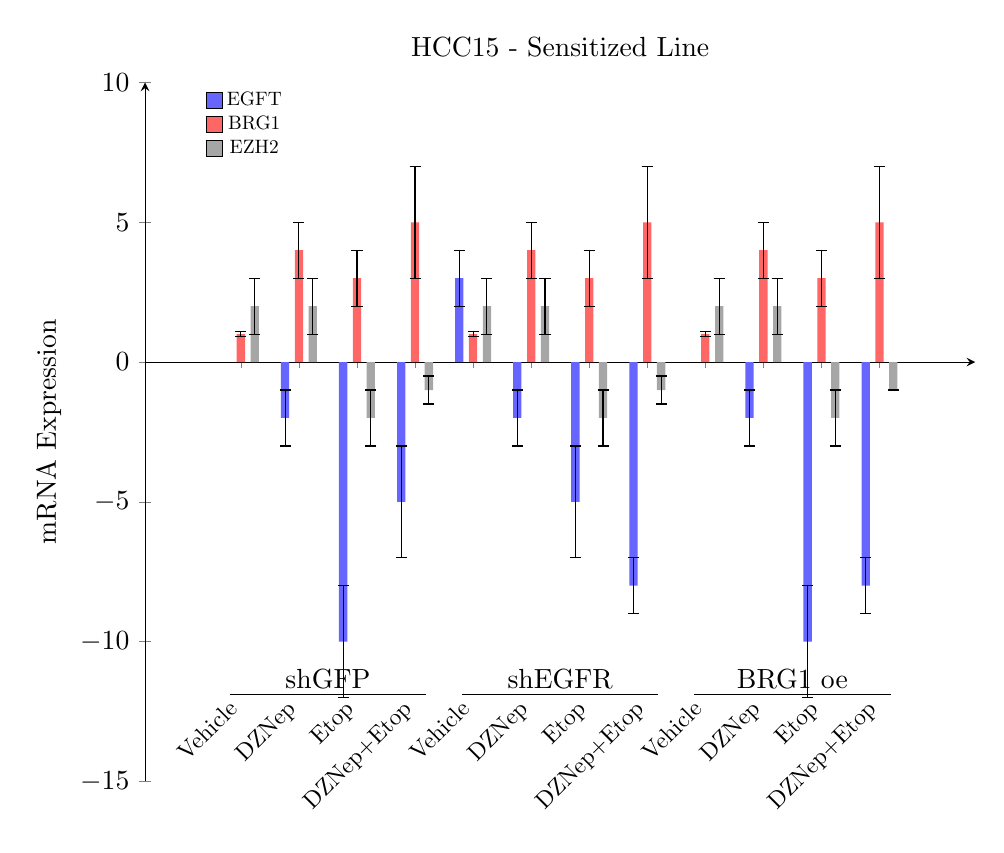
\begin{tikzpicture}
\newcounter{groupcnt}
% draw group line={<group column>}{<group value>}{<group label>}{<vertical offset>}{<line extension>}{<table name>}
\pgfplotsset{
    draw group line/.style n args={6}{
        after end axis/.append code={
            \setcounter{groupcnt}{0}
            \pgfplotstableforeachcolumnelement{#1}\of#6\as\cell{%
                \def\temp{#2}
                \ifx\temp\cell % if current row is in the group
                    \ifnum\thegroupcnt=0
                        \stepcounter{groupcnt}
                        \pgfplotstablegetelem{\pgfplotstablerow}{X}\of#6
                        \coordinate [yshift=#4] (startgroup) at (axis cs:\pgfplotsretval,0);
                    \else
                        \pgfplotstablegetelem{\pgfplotstablerow}{X}\of#6
                        \coordinate [yshift=#4] (endgroup) at (axis cs:\pgfplotsretval,0);
                    \fi
                \else % if we reach the end of current group
                    \ifnum\thegroupcnt=1
                        \setcounter{groupcnt}{0}
                        \draw [
                            shorten >=-#5,
                            shorten <=-#5
                        ] (startgroup) -- node [anchor=base, yshift=0.5ex] {#3} (endgroup);
                    \fi
                \fi
            }% end of for each column element
            \ifnum\thegroupcnt=1 % if we are at the end row
                        \setcounter{groupcnt}{0}
                        \draw [
                            shorten >=-#5,
                            shorten <=-#5
                        ] (startgroup) -- node [anchor=base, yshift=0.5ex] {#3} (endgroup);
            \fi
        }
    }
} % draw group line end -----------------

\pgfplotsset{my error bar/.style={
    error bars/.cd,y dir =both, y explicit,
  }
}

\pgfplotstableread{
X Gp  name EGFR EGFRerr BRG1 BRG1err EZH2 EZH2err
1 shGFP   Vehicle 0 0 1 0.1 2 1
2 shGFP   DZNep -2 1 4 1 2 1
3 shGFP   Etop -10 2 3 1 -2 1
4 shGFP   DZNep+Etop -5 2 5 2 -1 0.5
5 shEGFR  Vehicle 3 1 1 0.1 2 1
6 shEGFR  DZNep -2 1 4 1 2 1
7 shEGFR  Etop -5 2 3 1 -2 1
8 shEGFR  DZNep+Etop -8 1 5 2 -1 0.5
9  BRG1oe Vehicle 0 0 1 0.1 2 1
10 BRG1oe DZNep -2 1 4 1 2 1
11 BRG1oe Etop -10 2 3 1 -2 1
12 BRG1oe DZNep+Etop -8 1 5 2 -1 0.
}{\tabletwo}
\begin{axis}[
    width = \linewidth,
    title={HCC15 - Sensitized Line},
    ybar,
    bar width=3pt,
    axis x line = center, % change the default axis box.
    axis y line = left,
    enlarge x limits=0.15,
    ymin=-15, ymax=10,
    % legned related -------------
    legend image code/.code={
        \draw [#1] (0cm,-0.1cm) rectangle (0.2cm,0.1cm);
    },
    legend style={
        at={(0.18,1)},
        nodes={scale=0.7},
        draw = none     % without box
    },
    ylabel={mRNA Expression},
    % xtick related 
    xtick=data,
    xticklabels from table={\tabletwo}{name},
    xticklabel style={
        rotate=45,xshift=-85,yshift=-85,
        anchor=mid east,
        scale=0.85,
    },
    draw group line={Gp}{shGFP}{shGFP}{-120}{4pt}{\tabletwo},
    draw group line={Gp}{shEGFR}{shEGFR}{-120}{4pt}{\tabletwo},
    draw group line={Gp}{BRG1oe}{BRG1 oe}{-120}{4pt}{\tabletwo},
    ] % end of options of axis environment

% the "!" denotes the intensity
\addplot [draw=none, fill=blue!60,my error bar] table [y=EGFR,y error=EGFRerr] {\tabletwo};
\addplot [draw=none, fill=red!60,my error bar] table [y=BRG1,y error=BRG1err] {\tabletwo};
\addplot [draw=none, fill=gray!70,my error bar] table [y=EZH2,y error=EZH2err] {\tabletwo};

\legend{EGFT,BRG1,EZH2}

\end{axis}
\end{tikzpicture}

%\end{document}
    \caption{sub-figure from Extended Data Figure 8 in~\cite{2}.}
\end{figure}

\lipsum[1]
\begin{figure*}[tb]
  \centering
  %\documentclass[tikz]{standalone}
%\usepackage{pgfplots}
%\usetikzlibrary{calc}

% the figures style are inspired by \url{https://www.nature.com/articles/nature14122/figures/12}.
% For the use of draw group line, refer to https://tex.stackexchange.com/questions/55554/how-can-i-mix-an-ybar-and-an-ybar-stacked-with-pgfplots
%\begin{document}
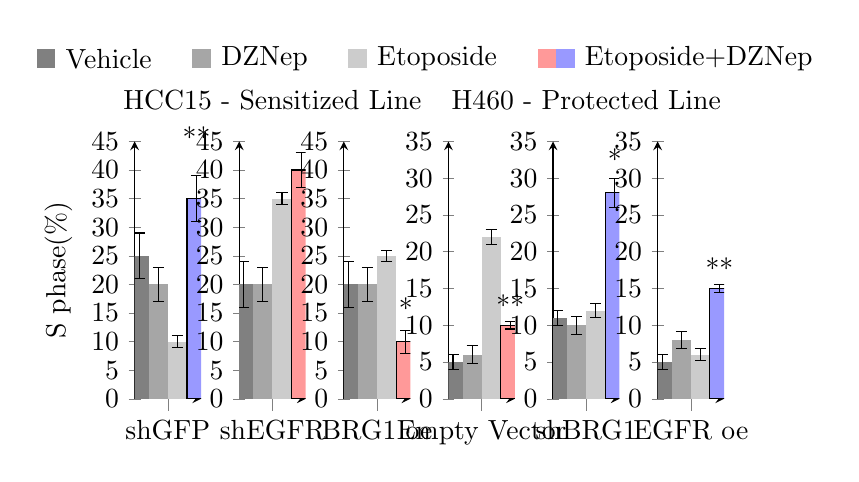
\begin{tikzpicture}
\pgfplotsset{my error bar/.style={error bars/.cd,y dir =both, y explicit}}
\pgfplotsset{
    subplotStyle/.style n args ={1}{
        axis x line = bottom, % change the default axis box.
        axis y line = left,
        width = 0.2\linewidth ,
        height = 0.4\linewidth ,
        ybar=0,
        bar width = 0.02\linewidth ,
        ytick={0,5,...,45},
        ymin=0,ymax=45,
        nodes={scale=1},
        xtick=data,
    }
}
\newcommand{\subplotxoffset}{.04\linewidth}
% plot1 ---------------------------
\newcommand{\subplotName}{shGFP}
\begin{axis}[
    name=plot1,
    ylabel=S phase(\%),
    symbolic x coords={\subplotName},
    subplotStyle={45},
]

\addplot [draw=none,fill=gray!100,my error bar] coordinates {(\subplotName,25)+-(0,4)};
\addplot [draw=none,fill=gray!70,my error bar] coordinates {(\subplotName,20)+-(0,3)};
\addplot [draw=none,fill=gray!40,my error bar] coordinates {(\subplotName,10)+-(0,1)};
\addplot [
    nodes near coords={**},
    nodes near coords style = {
       yshift=15pt,xshift=0pt,
    },
    fill=blue!40,
    my error bar,
    ] coordinates {(\subplotName,35)+-(0,4)};
\end{axis}

% plot2 ----------------------------
\renewcommand{\subplotName}{shEGFR}
\begin{axis}[
    name=plot2,
    at = {($(plot1.east)+(\subplotxoffset,0)$)},
    anchor=west,
    %enlargelimits=0.05,
    symbolic x coords={\subplotName},
    subplotStyle={45},
]
\addplot [draw=none,fill=gray!100,my error bar] coordinates {(\subplotName,20)+-(0,4)};
\addplot [draw=none,fill=gray!70,my error bar] coordinates {(\subplotName,20)+-(0,3)};
\addplot [draw=none,fill=gray!40,my error bar] coordinates {(\subplotName,35)+-(0,1)};
\addplot [fill=red!40,my error bar] coordinates {(\subplotName,40)+-(0,3)};
\end{axis}

% plot3 --------------------------------
\renewcommand{\subplotName}{BRG1 oe}
\begin{axis}[
    name=plot3,
    at = {($(plot2.east)+(\subplotxoffset,0)$)},
    anchor=west,
    %enlargelimits=0.05,
    symbolic x coords={\subplotName},
    subplotStyle={45},
]
\addplot [draw=none,fill=gray!100,my error bar] coordinates {(\subplotName,20)+-(0,4)};
\addplot [draw=none,fill=gray!70,my error bar] coordinates {(\subplotName,20)+-(0,3)};
\addplot [draw=none,fill=gray!40,my error bar] coordinates {(\subplotName,25)+-(0,1)};
\addplot [
    nodes near coords={*},
    nodes near coords style = {
       yshift=5pt,xshift=0pt,
    },
    fill=red!40,my error bar
    ] coordinates {(\subplotName,10)+-(0,2)};
\end{axis}

\renewcommand{\subplotName}{Empty Vector}
\begin{axis}[
    name=plot4,
    at = {($(plot3.east)+(\subplotxoffset,0)$)},
    anchor=west,
    %enlargelimits=0.05,
    symbolic x coords={\subplotName},
    subplotStyle={45},
    ymax=35,
]
\addplot [draw=none,fill=gray!100,my error bar] coordinates {(\subplotName,5)+-(0,1)};
\addplot [draw=none,fill=gray!70,my error bar] coordinates {(\subplotName,6)+-(0,1.2)};
\addplot [draw=none,fill=gray!40,my error bar] coordinates {(\subplotName,22)+-(0,1)};
\addplot [
    nodes near coords={**},
    nodes near coords style = {
       yshift=0pt,xshift=0pt,
    },
    fill=red!40,my error bar] 
    coordinates {(\subplotName,10)+-(0,0.5)};
\end{axis}

% plot5 -----------------------------------
\renewcommand{\subplotName}{shBRG1}
\begin{axis}[
    name=plot5,
    at = {($(plot4.east)+(\subplotxoffset,0)$)},
    anchor=west,
    %enlargelimits=0.05,
    symbolic x coords={\subplotName},
    subplotStyle={45},
    ymax=35,
]
\addplot [draw=none,fill=gray!100,my error bar] coordinates {(\subplotName,11)+-(0,1)};
\addplot [draw=none,fill=gray!70,my error bar] coordinates {(\subplotName,10)+-(0,1.2)};
\addplot [draw=none,fill=gray!40,my error bar] coordinates {(\subplotName,12)+-(0,1)};
\addplot [
    nodes near coords={*},
    nodes near coords style = {
       yshift=5pt,xshift=0pt,
    },
    fill=blue!40,my error bar
    ] coordinates {(\subplotName,28)+-(0,2)};
\end{axis}

% plot6 -----------------------------------
\renewcommand{\subplotName}{EGFR oe}
\begin{axis}[
    name=plot6,
    at = {($(plot5.east)+(\subplotxoffset,0)$)},
    anchor=west,
    %enlargelimits=0.05,
    symbolic x coords={\subplotName},
    subplotStyle={45},
    ymax=35,
    %% the legends to be placed outside 
    legend image code/.code={
        \draw [#1] (0cm,-0.1cm) rectangle (0.2cm,0.1cm);
    },
    legend style={
        legend columns=-1,
        draw=none,
        fill=none,
    },
    legend entries={Vehicle,DZNep,Etoposide,Etoposide+DZNep},
    legend to name=commonLegendb,
]
\addplot [draw=none,fill=gray!100,my error bar] coordinates {(\subplotName,5)+-(0,1)};
\addplot [draw=none,fill=gray!70,my error bar] coordinates {(\subplotName,8)+-(0,1.2)};
\addplot [draw=none,fill=gray!40,my error bar] coordinates {(\subplotName,6)+-(0,0.8)};
\addplot [
    nodes near coords={**},
    nodes near coords style = {
       yshift=0pt,xshift=0pt,
    },
    fill=blue!40,my error bar
    ] 
    coordinates {(\subplotName,15)+-(0,0.5)};
\end{axis}
%% end of the plots ----------------------

% plot the title for the two groups
\node [scale=1] (title1) at ($(plot1.north)!0.5!(plot3.north)+(0,15pt)$) {HCC15 - Sensitized Line};
\node [scale=1] (title2) at ($(plot4.north)!0.5!(plot6.north)+(0,15pt)$) {H460 - Protected Line};

% self draw the legend ---------------
\node [matrix,fill=none,draw=none] (mylegendnode) at ($(title1.north)!0.5!(title2.north)+(0,8pt)$)
{
\node [fill=gray!100,shape=rectangle,label=right:Vehicle]{}; &[4mm]
\node [fill=gray!70,shape=rectangle,label=right:DZNep]{}; &[4mm]
\node [fill=gray!40,shape=rectangle,label=right:Etoposide]{}; &[4mm]
\node [fill=red!40,shape=rectangle]{}; &
\node [fill=blue!40,shape=rectangle,label=right:Etoposide+DZNep]{}; \\
};

% draw legend with pgfplot function (Not work well)--------------
%\node [scale=0.8] (mylegendnode) at ($(title1.north)!0.5!(title2.north)+(0,8pt)$) {\pgfplotslegendfromname{commonLegendb}};

\end{tikzpicture}

%\end{document}
  \caption{sub-figure from Extended Data Figure 8 in~\cite{2}.}
\end{figure*}

\lipsum
\lipsum[1]
% figure 1 ------------------------------------------
\begin{figure*}[htb]
    \begin{center}
        %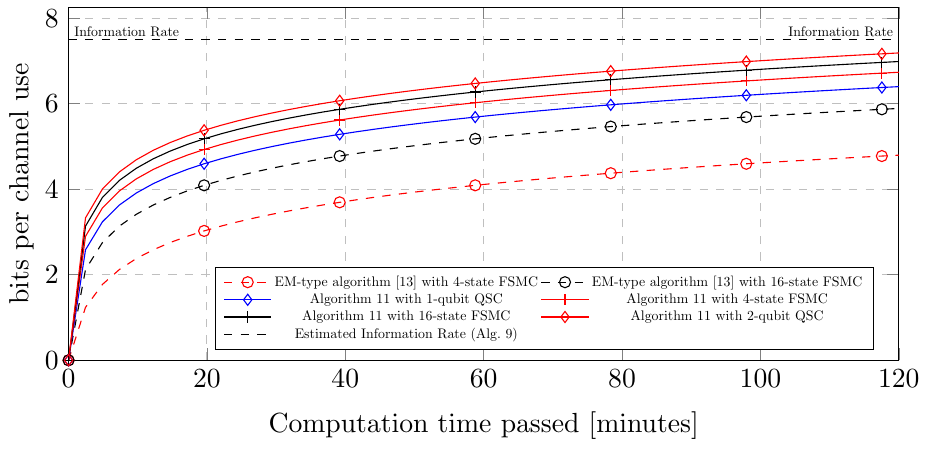
\includegraphics[width=.8\linewidth]{submodules/1/1.pdf}
        % style from fig.11 in https://ieeexplore.ieee.org/abstract/document/9031358
\begin{tikzpicture}
\pgfplotstableread{submodules/1/datafile1.csv}{\datatable}
\begin{axis}[
  xlabel={Computation time passed~[minutes]},
  ylabel={bits per channel use},
  ylabel style={at={(axis description cs:0.03,0.5)}},
  xmin= 0, xmax= 120, ymin= 0,
  legend style = {
      legend pos=south east,
      legend columns = {2},
      nodes={scale=0.8}, % make the legend box smaller
      %font = {\tiny},
  },
  grid = major,
  grid style=dashed,
  mark repeat={8},
  width = \linewidth,
  height = 0.4\linewidth,
  mark options={solid},
  %% extra label for information rate
  every axis/.append style={
      extra description/.code={
          \node[scale=0.85] at (0.08,0.94) {Information Rate};
          \node[scale=0.85] at (0.92,0.94) {Information Rate};
      },
  },
] % end of axis setting

  %1
  \addplot[red,mark=o,dashed] table [x index=0, y index=1] {\datatable};
  \addlegendentry{EM-type algorithm~[13] with 4-state FSMC}

  %2
  \addplot[dashed,mark=o] table [x index=0, y index=2] {\datatable};
  \addlegendentry{EM-type algorithm~[13] with 16-state FSMC}

  %3
  \addplot[blue,mark=diamond] table [x index=0, y index=3] {\datatable};
  \addlegendentry{Algorithm~11 with 1-qubit QSC}

  %4
  \addplot[red,mark=+] table [x index=0, y index=4] {\datatable};
  \addlegendentry{Algorithm~11 with 4-state FSMC}

  %5
  \addplot[mark=+] table [x index=0, y index=5] {\datatable};
  \addlegendentry{Algorithm~11 with 16-state FSMC}

  %6
  \addplot[red,mark=diamond] table [x index=0, y index=6] {\datatable};
  \addlegendentry{Algorithm~11 with 2-qubit QSC}

  %7
  \addplot[dashed] table [x index=0, y index=7] {\datatable};
  \addlegendentry{Estimated Information Rate~(Alg.~9)}

\end{axis}
\end{tikzpicture}
    \end{center} 
    \caption{This is fig.11 from~\cite{1}}
\end{figure*}

% figure 3a/3b -----------------------------
\lipsum
\begin{figure*}[htb]
  \centering
  
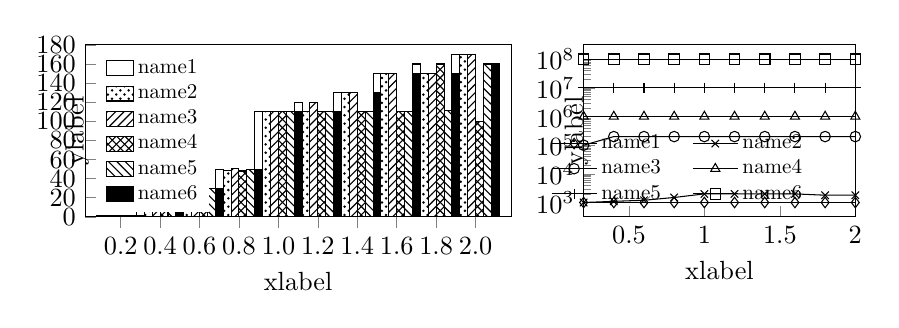
\begin{tikzpicture}[scale=0.95]
\pgfplotstableread{
budget    name1   name2   name3   name4    name5    name6
0.2 1   1   1   1   1   1
0.4 10  10  10  10  10  10
0.6 30  30  30  30  30  30 
0.8 50  49  51  48  50  50
1.0 110 110 110 110 110 110
1.2 120 110 120 110 110 110
1.4 130 130 130 110 110 130
1.6 150 150 150 110 110 150
1.8 160 150 150 160 111 150
2.0 170 170 170 100 160 160
}{\datatablea}

\pgfplotstableread{
X   name1   name2   name3   name4   name5   name6
0.2 1e3 1e3 1e5 1e6 1e7 1e8
0.4 1e3 1.1e3 2e5 1e6 1e7 1e8
0.6 1e3 1.2e3 2e5 1e6 1e7 1e8
0.8 1e3 1.5e3 2e5 1e6 1e7 1e8
1.0 1e3 2e3 2e5 1e6 1e7 1e8
1.2 1e3 2e3 2e5 1e6 1e7 1e8
1.4 1e3 2e3 2e5 1e6 1e7 1e8
1.6 1e3 2e3 2e5 1e6 1e7 1e8
1.8 1e3 1.8e3 2e5 1e6 1e7 1e8
2.0 1e3 1.8e3 2e5 1e6 1e7 1e8
}{\datatableb}
% table read done. ----------------------------

%% fig a ------------------------------------
\begin{axis}[
  name=leftplot,
  width = .6\linewidth, height = 0.32\linewidth,
  %title={The Title},
  title style={at={(0.5,-0.35)}},
  xtick pos=bottom,
  ytick pos=left, % remove the tick from the right and top
  ybar=0,
  ylabel={ylabel},
  ylabel style={at={(axis description cs:0.03,0.5)}},
  ytick={0,20,...,180},
  bar width=3pt,
  %enlarge x limits=0.15,
  ymin=0, ymax=180,
  % legned related -------------
  legend image code/.code={
      \draw [#1] (0cm,-0.1cm) rectangle (0.35cm,0.1cm);
  },
  legend style={
      %at={(0.13,1)},
      legend pos=north west,
      nodes={scale=0.8},
      draw = none,        % without box
      cells={anchor=west}, % algin left
  },
  xlabel={xlabel},
  % xtick related 
  xtick=data,
  xticklabels from table={\datatablea}{budget},
  %xticklabel style={
  %j    rotate=45,xshift=-100,yshift=-100,anchor=mid east
  %j},
] % end of options of axis environment

\newcommand{\mysubplot}[2]{
    \addplot[#2] table [x=budget,y=#1] {\datatablea};
    \addlegendentry{#1};
}
\mysubplot{name1}{}
\mysubplot{name2}{pattern=crosshatch dots}
\mysubplot{name3}{pattern=north east lines}
\mysubplot{name4}{pattern=crosshatch}
\mysubplot{name5}{pattern=north west lines}
\mysubplot{name6}{fill=black}

\end{axis}

%% fig b --------------------------

\begin{axis}[
  at={($(leftplot.east)+(.08\linewidth,0)$)},
  anchor=west,
  xlabel={xlabel},
  ylabel={ylabel},
  ylabel style={at={(axis description cs:0.05,0.5)}},
  xmin= 0.2, xmax= 2.0, 
  legend style = {
      at={(0.35,0.28)},
      anchor=center,
      legend columns = {2},
      nodes={scale=0.8}, % make the legend box smaller
      fill=none,
      draw=none,
      /tikz/every even column/.append style={column sep=.03\linewidth},
  },
  width = .43\linewidth,
  height = 0.32\linewidth,
  mark options={solid},
  ymode=log, % the log scale
  ytick={1e3,1e4,1e5,1e6,1e7,1e8},
  ytick pos=left, % remove the tick from the right and top
  xtick pos=bottom,
]
    \newcommand{\mysubplot}[2]{
        \addplot [#2] table [x=X,y=#1] {\datatableb};
        \addlegendentry{#1};
    }
    \mysubplot{name1}{mark=diamond}
    \mysubplot{name2}{mark=x}
    \mysubplot{name3}{mark=o}
    \mysubplot{name4}{mark=triangle}
    \mysubplot{name5}{mark=+}
    \mysubplot{name6}{mark=square}

\end{axis}
\end{tikzpicture}
  \caption{(A figure across two columns)}
\end{figure*}

%% fig4 -------------------------------
\lipsum
\begin{figure*}[htb]
  \begin{center}
  \documentclass[tikz]{standalone}
\usepackage{pgfplots}
\usepgfplotslibrary{fillbetween}
\usetikzlibrary{calc}
%% refer to fig4 in https://papers.nips.cc/paper/2020/file/83eaa6722798a773dd55e8fc7443aa09-Paper.pdf

\begin{document}
\begin{tikzpicture}

% \plotdata{number}{color}{other options}
\newcommand{\plotdata}[3]{
  \addplot[#2,#3,line width=.6pt] table [x=X, y=data#1] {\datatable};
  
  \addplot[name path=A#1, draw=none,forget plot] table [x=X, y=data#1l] {\datatable};
  \addplot[name path=B#1, draw=none,forget plot] table [x=X, y=data#1u] {\datatable};
  \addplot[#2!20,forget plot] fill between[of=A#1 and B#1]; 
}
% read the external table
\pgfplotstableread[col sep=comma]{datafile1.csv}{\datatable}
\pgfplotsset{
  title style={
    at={(0.5,-0.25)},
    align=left, 
    anchor=north,
  },
  subplotStyle/.style n args ={1}{
      smooth, no markers,
      width = 0.4\linewidth,
      height = 0.35\linewidth,
      axis x line=bottom,
      axis y line=left,
      enlargelimits=auto,
      xmin=0,
  },
}
\newcommand{\subplotoffset}{0.05\linewidth}
\newcommand{\mygreen}{green!60!black}

%% plot1 ------------------------------
\begin{axis}[
    name=plot1,
    title={(a) Single-circle},
    ylabel={Root\\ Mean\\ Squared\\ Error\\ Averged\\ Over\\ 20runs},
    ylabel style={
      rotate=-90,
      anchor=center,
      align=center,
      scale={0.7},
      at={(0.1,0.5)},
    },
    legend entries={Implicit,MDN-3,MDN-4,MDN-6,KDE},
    legend columns=-1,
    legend style={
      fill=none,
    },
    legend to name={legendName},
    subplotStyle={},
]
\plotdata{1}{red}{}
\plotdata{2}{\mygreen}{}
\plotdata{3}{\mygreen}{dotted}
\plotdata{4}{\mygreen}{dashdotted}
\addplot[blue,line width=.6pt] coordinates  {(0,0.5) (100,0.5)};
\end{axis}

%% plot2 --------------------------
\begin{axis}[
  name=plot2,
  at={($(plot1.east)+(\subplotoffset,0)$)},
  anchor=west,
  title={(b) Double-circle},
  subplotStyle={},
]
\plotdata{5}{red}{}
\plotdata{6}{\mygreen}{}
\plotdata{7}{\mygreen}{dotted}
\plotdata{8}{\mygreen}{dashdotted}
\addplot[blue,line width=.6pt] coordinates  {(0,1) (100,1)};
\end{axis}

%% plot3 ------------------------------------
\begin{axis}[
  name=plot3,
  at={($(plot2.east)+(\subplotoffset,0)$)},
  anchor=west,
  title={(c) High-dimentional \\Double-circle},
  subplotStyle={},
]
\plotdata{5}{red}{}
\plotdata{6}{\mygreen}{}
\plotdata{7}{\mygreen}{dotted}
\plotdata{8}{\mygreen}{dashdotted}
\addplot[blue,line width=.6pt] coordinates  {(0,4) (100,4)};
\end{axis}

\node [] (mylegendnode) at ($(plot1.south)!0.5!(plot3.south)+(0,-0.15\linewidth)$) {\pgfplotslegendfromname{legendName}};
%\ref{legendName}
\end{tikzpicture}
\end{document}

  \end{center}
  \caption{\lipsum[1]}
\end{figure*}

% usage \includeSubmodule{name}{additional caption}{*?}
\newcommand{\includeSubmodule}[3]{
    \begin{figure#3}[!htb]
        \begin{center}
            \includegraphics[width=\linewidth]{submodules/#1/#1.pdf}
        \end{center} 
        \caption{#2}
    \end{figure#3}
}

\lipsum[1]
%\includeSubmodule{4}{pcode example}{}
%\documentclass[varwidth]{standalone}
%\usepackage[ruled,linesnumbered]{algorithm2e}
%\usepackage{xcolor}
%
%\begin{document}

\begin{algorithm}[h]
%\SetAlgoLined 
\SetAlgoVlined % Remove the end for each block . you can also use vlined in option of package algorithm2e
\DontPrintSemicolon
\newcommand\mycommfont[1]{\textcolor{blue}{#1}}
\SetCommentSty{mycommfont} % change the comment style

\caption{Example code}
\KwIn{Your Input}
\KwOut{Your output}
\KwData{Testing set x}
$\sum_{i=1}^{\infty}:=0$ \tcp*{this is a comment}
\tcc{Now this is an if...else conditional loop}
\If{Condition 1}{
    Do something \tcp*{this is another comment}
    \If{sub-Condition}{
        Do a lot \;
    }
}
\ElseIf{Condition 2}{
    Do Otherwise\;
    \tcc{Now this is a for loop}
    \For{sequence}{
        loop instructions\;
    }
}
\Else{
    Do the rest\;
}
\tcc{Now this is a While loop}
\While{Condition}{
    Do somthing\;
}
 
\end{algorithm}
%\end{document}
 %% pcode
\lipsum
%\includeSubmodule{6}{table example 02}{*}
\includeSubmodule{5}{table example 01}{*} 
\lipsum[1]

\newcommand{\xmark}{\ding{55}}%package pifont
\begin{table}[h]
  \centering
  \begin{tabular}{|c|c|c|c|}
    \hline
    Paper & Route Planning & Speed Planning & Hard Deadline \\  \hline
    [37] & \checkmark & \xmark & \xmark \\ \hline
    [16] & \xmark & \checkmark & \xmark \\ \hline
    [17] & \xmark & \checkmark &  \checkmark \\ \hline
    This work & \checkmark&\checkmark & \checkmark\\ \hline
  \end{tabular}
  \caption{Table~II from~\cite{deng2017energy}}
\end{table}
\lipsum

%%% table ------------------------------
\begin{table}[htb]
    \caption{Population variation in hatch success(mean percent) of unfertilized eggs for females from populations sampled in 1997.}
    \begin{tabularx}{\linewidth}{lXXXr}
        \hline  \\[-10pt]
        Population & mean (\%)  &\begin{tabular}[c]{@{}l@{}}Standard\\ deviation\end{tabular}   & Range & N  \\ \hline
        Population name1$^T$ & 10 & 1 & 0-50 & 10 \\ 
        Population name2$^T$ & 10 & 1 & 0-50 & 10 \\ 
        Population name3$^T$ & 10 & 1 & 0-50 & 10 \\ 
        Population name4$^P$ & 10 & 1 & 0-50 & 10 \\ 
        Population name5$^P$ & 10 & 1 & 0-50 & 10  \\ 
        Population name6$^P$ & 10 & 1 & 0-50 & 10 \\ 
        Population name7$^L$ & 10 & 1 & 0-50 & 10 \\ 
        Population name8$^L$ & 10 & 1 & 0-50 & 10 \\ 
        Population name9$^L$ & 10 & 1 & 0-50 & 10 \\ 
        \hline 
    \end{tabularx}
    \begin{tablenotes}
    \item $\leftidx{^T}{}$ = \footnotesize{temporary stream},
    $\leftidx{^P}{}$ = \footnotesize{permanent streams}, 
    $\leftidx{^L}{}$ = \footnotesize{lakes}.
    \item
    \item 
    \end{tablenotes}
\end{table}
\lipsum

\bibliographystyle{unsrt}
\bibliography{ref}
\end{document}